\documentclass{beamer}
\mode<presentation>
{ \usetheme{boxes} }

\usepackage{times}
\usepackage{acronym}
\usepackage{graphicx}
\usepackage{csquotes}
\usepackage[UKenglish]{babel}
\usepackage[backend=bibtex]{biblatex}

\newcommand{\etal}{\textit{et al}. }
\newcommand{\ie}{\textit{i}.\textit{e}., }
\newcommand{\eg}{\textit{e}.\textit{g}. }
\newcommand{\etc}{\textit{etc}. }

\title{Variability and Transformations}
\author{Marco Craveiro}
\date{\today}

\AtBeginSection[]
{
  \begin{frame}<beamer>
    \frametitle{Outline}
    \tableofcontents[currentsection]
  \end{frame}
}

\bibliography{variability_and_transformations}

\begin{document}

\begin{frame}

\titlepage{}

% v${DOGEN_VERSION} % chktex-file 25

\end{frame}

\section{\ac{MDE}}

\begin{frame}
\frametitle{What is \ac{MDE}}

\begin{itemize}
\item The previous presentation provided an overview of what \acf{MDE}
  is and why you should consider it for Software Engineering. Let's do
  a quick recap.

\pause{}

\item \ac{MDE} is a \enquote{development paradigm that uses models as
  the primary artifact of the development process. Usually [\ldots]
  the implementation is (semi-) automatically generated from the
  models.}\cite{brambilla2012model}

\pause{}

\item \ac{MDE} ``goes beyond the pure development activities and
  encompasses other model-based tasks of a complete software
  engineering process (\eg the model-based evolution of the system or
  the model-driven reverse engineering of a legacy
  system.)''\cite{brambilla2012model}

\pause

\item ``Fundamental'' \ac{MDE} equation: Models + Transformations =
  Software

\end{itemize}

\end{frame}

\begin{frame}
\frametitle{\ac{MDE} Key Components: Models}

\begin{itemize}

\item \ac{MDE} is only interested in a special class of models: those
  which are described according to a \textbf{formal language} and thus
  have precise semantics.

\pause

\item Formal models are written using a \acf{DSL}. The \ac{DSL} is
  designed specifically for modeling.

\pause

\item \acf{UML} is an example of such a \ac{DSL} (\emph{when suitably
  extended with stereotypes and profiles}). \ac{UML} has a graphical
  representation~--- called a \emph{concrete syntax}~--- but it also
  has an \emph{abstract syntax}.

\pause

\item A \emph{meta-model} is made up of the abstract syntax and the
  static semantics of the \ac{DSL}. The metamodel is the basis for
  \emph{transformations}.

\end{itemize}

\end{frame}

\begin{frame}
\frametitle{\ac{MDE} Key Components: Transforms}

\begin{itemize}
\item \emph{Transformations}~--- or just transforms~--- can be thought
  of as functions that take models as inputs and produce an output.

\pause

\item We can classify transforms based on the \emph{type} of its
  output:

\pause

\begin{itemize}

\item \textbf{\acf{M2M}}: the output is another model. Note that the
  output can \emph{conform} to the same metamodel or to a different
  metamodel.

\pause

\item \textbf{\acf{M2T}}: the output is a textual representation of
  the model.

\end{itemize}

\pause

\item \ac{M2T} transforms are commonly referred to as
  \emph{generators} because they generalise of the notion of a
  \emph{code generator}.

\end{itemize}

\end{frame}

\section{\acf{SPL}}

\begin{frame}
\frametitle{What are \ac{SPL}}

\begin{itemize}

\item \ac{MDE} ``pursues the goal of creating a software
  \emph{product} in part or in the whole through one or more
  transformations.''\cite{volter2013model}

\pause

\item Once you have a product, the next logical think is to think of
  \emph{product families}: ``the set of all products that can be
  created with a certain domain architecture is commonly referred to
  as a \emph{software system family}.''\cite{volter2013model}

\pause

\item ``Software product line engineering aims to reduce development
  time, effort, cost, and complexity by taking advantage of the
  commonality within a portfolio of similar
  products.''\cite{voelter2007handling}

\end{itemize}

\end{frame}

\begin{frame}
\frametitle{What are \ac{SPL}}

\begin{itemize}

\item ``The main idea of software product lines is to design a family
  of systems instead of one single system. A family of systems defines
  a set of systems that share substantial commonalities but also
  exhibit explicit variations.''\cite{brambilla2012model}

\pause

\item In theory, \acf{PLE} integrates well with \ac{MDE}: it provides
  an analytical framework with which to model the domain looking for
  variations.

\pause

\item If all went according to plan, we should be able to ``simply''
  supply additional inputs to our models; these then determine the
  \emph{concrete} product we want to produce from the universe of
  \emph{possible} products supported by our models. The key here is
  \emph{variability} and how to express it.

\end{itemize}

\end{frame}

\section{Variability}

\begin{frame}
\frametitle{Variability}

\begin{itemize}

\item ``Variability management is the activity concerned with
  identifying, designing, implementing, and tracing flexibility in
  software product lines (SPLs).''\cite{voelter2007handling}

\pause

\item ``The effectiveness of a software product line approach directly
  depends on how well feature variability within the portfolio is
  implemented and managed throughout the development lifecycle, from
  early analysis through maintenance and
  evolution.''\cite{groher2007expressing}

\end{itemize}

\end{frame}

\begin{frame}
\frametitle{Variability}

In practice, there are problems integrating \ac{MDE} with
\ac{PLE}. Brambilla states\cite{brambilla2012model}:

\begin{quote}
One of the most interesting question [sic] when it comes to software
product lines and model driven engineering is how to formulate the
knowledge of a \ac{SPL} by using models. Especially, the variability
aspect is in this context of main interest as modeling languages are
quite often lacking variability as a first-class language concept
\end{quote}

\end{frame}

\begin{frame}
\frametitle{Traditional Handling of Variability}

\begin{itemize}

\item Thus far, Software Engineers have handled variability using the
  available tools:

  \pause

  \begin{itemize}

  \item mechanisms provided by the implementation language: patterns,
    frameworks, polymorphism, reflection, pre-compilers,
    pre-processors.

    \pause

  \item configuration and build tools to set compile time variables
    and select variants of assets.

  \end{itemize}

  \pause

\item These approaches are limited because they are at the wrong level
  of abstraction: the code.

\pause

\item In the context of \ac{MDE} and \ac{SPL} we want to make the most
  of variability as a first class citizen.

\end{itemize}

\end{frame}

\begin{frame}
\frametitle{Feature Models}

One possible solution is to use a metamodel designed specifically to
model variability. A common choice is the Feature
Model\cite{czarnecki2000generative}:

\begin{figure}
  \centering
  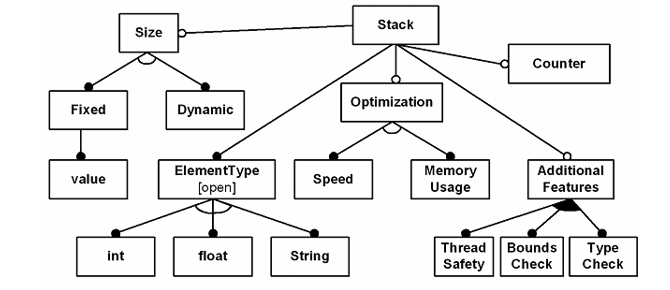
\includegraphics[scale=0.4]{images/example_feature_model_voelter.png}
  \caption{Example feature model.\cite{groher2007expressing}}
\end{figure}

\end{frame}

\begin{frame}
\frametitle{Feature Models}

\begin{itemize}

\item By using a feature model, we now have a much more intuitive way
  to define the features and their relationships; the language was
  defined specifically to have the vocabulary to do so. But\ldots

  \pause

\item \ldots as JWZ famously said: \enquote{Some people, when
  confronted with a problem, think \enquote{I know, I'll use regular
    expressions.} Now they have two problems.}

  \pause

\item The question then is: how do we integrate the traditional
  \ac{MDE} modeling techniques~--- based on modeling \ac{DSL}s~---
  with the modeling of variability? Groher and V{\"o}lter propose a
  solution to this ``two-model'' problem in their papers.

\end{itemize}

\end{frame}

\begin{frame}
\frametitle{Variability Pervasiveness}

First we need to understand more about the nature of variability. The
trouble is, variability is \emph{pervasive}; it exists at all levels
of \ac{MDE}, from analysis, to problem space, to solution space:

\pause

\begin{itemize}
\item Variability impacts \emph{all} the models we create: some
  model elements may be added or removed depending how we choose to
  instantiate the product;

  \pause

\item Variability impacts \ac{M2M} transforms: they may require
  parameters expressing user choices in order to execute;

  \pause

\item Variability impacts \ac{M2T} transforms: some code may or may
  not be generated in response to user choices.

\end{itemize}

\end{frame}

\begin{frame}
\frametitle{Variability Classification}

\begin{itemize}

\item Groher and V{\"o}lter classify variability into two broad
  types\cite{groher2007expressing}:

\pause

\begin{itemize}
\item \textbf{Structural}: described using creative construction DSLs,
  \eg \ac{UML}. These allow one to creatively construct any arbitrary
  data structure, defining any number of models.

\pause

\item \textbf{Non-structural}: described using configuration
  languages, \eg application config files, build system configuration,
  macros, \etc

\pause

\end{itemize}

\item Their focus is on structural variability.

\end{itemize}

\end{frame}

\begin{frame}
\frametitle{Variability Classification}

In practice, variability does not fit neatly into these
categories. Instead, there is a ``spectrum of languages commonly used
for expressing and binding variability.''\cite{groher2007expressing}

\begin{figure}
  \centering
  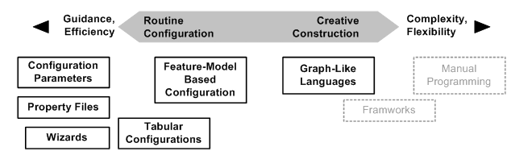
\includegraphics[scale=0.6]{images/variability_spectrum_voelter.png}
  \caption{Expressive power of \ac{DSL}s.\cite{groher2007expressing}}
\end{figure}

\end{frame}

\begin{frame}
\frametitle{Approach}

Now we have enough context, we can focus on the overall approach. It
can be summarised as follows:

\pause

\begin{itemize}

\item ``[Use] models to describe product lines. Variants are defined
  on [sic] model-level.  Transformations generate running
  applications. \acf{AO} techniques are used to help define the
  variants in the models as well as in the transformers and
  generators.''\cite{voelter2007handling}

  \pause

\item ``The core idea is to express variability in models and
  generators, since, due to the higher abstraction level in models
  [\ldots], the number of variation points is
  lower[\ldots].''\cite{voelter2007handling}

\end{itemize}

\end{frame}

\begin{frame}
\frametitle{Approach}

We can see this visually:

\begin{figure}
  \centering
  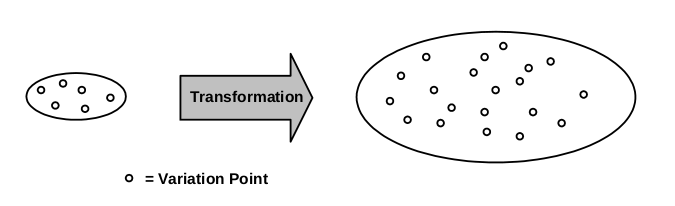
\includegraphics[scale=0.5]{images/variation_point_voelter.png}
  \caption{Variation points in
    models\ac{DSL}s.\cite{voelter2007handling}}
\end{figure}

\end{frame}

\begin{frame}
\frametitle{Implementation Approach}

\begin{itemize}

\item Groher and V{\"o}lter was to ``divide and conquer''. They split
  variability into two types, from an implementation perspective:
  \emph{Positive Variability} and \emph{Negative Variability}. Details
  on next slide.

  \pause

\item For each variability type they created specific tooling. They
  extended an existing modeling toolchain with these additional tools.

  \pause

  \item They had to create changes at all levels: from feature
    modeling, to transformation workflows, to the generator templates.

\end{itemize}

\end{frame}

\begin{frame}
\frametitle{Positive Variability}

``[S]tarts with a minimal core and selectively adds additional parts
based on the presence or absence of features in the configuration
models.''\cite{groher2007expressing} In this case we need to
\emph{weave} in other models in response to user choices.

\pause

\begin{figure}
  \centering
  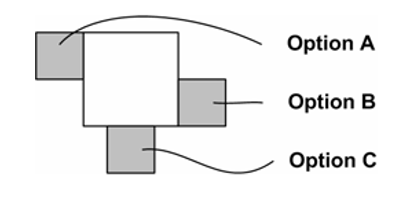
\includegraphics[scale=0.3]{images/positive_variability_voelter.png}
  \caption{Positive variability.\cite{groher2007expressing}}
\end{figure}

\end{frame}

\begin{frame}
\frametitle{Negative Variability}

``Negative variability selectively takes away parts of a creative
construction model based on the presence or absence of features in the
configuration models.''\cite{groher2007expressing} In this case we
need to remove model elements in response to user choices.

\pause

\begin{figure}
  \centering
  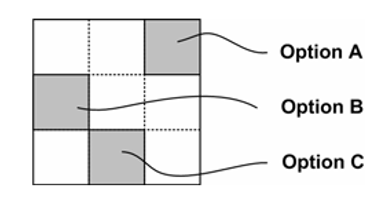
\includegraphics[scale=0.5]{images/negative_variability_voelter.png}
  \caption{Negative variability.\cite{groher2007expressing}}
\end{figure}

\end{frame}

\begin{frame}

\begin{center}
  \huge{Thank You}
\end{center}

\end{frame}

\begin{frame}

\begin{center}
    \huge{Q \& A}
\end{center}

\end{frame}

\begin{frame}
\frametitle{Acronyms}

\begin{acronym}
  \acro{AO}{Aspect Oriented}
  \acro{DSL}{Domain Specific Language}
  \acro{GPML}{General Purpose Modeling Languages}
  \acro{M2M}{Model-to-Model}
  \acro{M2T}{Model-to-Text}
  \acro{MDE}{Model Driven Engineering}
  \acro{PIM}{Platform Independent Model}
  \acro{PLE}{Product Line Engineering}
  \acro{PSM}{Platform Specific Model}
  \acro{SPL}{Software Product Lines}
  \acro{T2M}{Text-to-Model}
  \acro{UML}{Unified Modeling Language}
\end{acronym}

\end{frame}

\begin{frame}
\frametitle{Bibliography}

\printbibliography

\end{frame}

\end{document}
